%!TEX root = ../../main.tex

% TODO: Input chapters here that the readers will have to read in order to understand the base for the rest of the document

\noindent When referring to the ``\giraf-software suite'' throughout the manual, we mean the entire \giraf project being developed by the current Software 6 semester at Aalborg University. This extends to all the individual applications and their dependency applications being developed, which at the current time of writing includes: 

\begin{itemize}
    \item Giraf (Main Launcher)
    \item Administration (Profile Manager)
    \item Sekvens (Sequence)
    \item Ugeplan (Week Schedule)
    \item Piktosearch (Picto Search)
    \item Pictooplæser (Picto Reader)
    \item Kategoriværktøjet (Category Manager)
    \item Kategorispillet (Category Game)
    \item Tidstager (Timer)
    \item Livshistorier (Life Story)
    \item Stemmespillet (Voice Game)
\end{itemize}

%!TEX root = ../../main.tex
\chapter{Box Model}
\label{cha:box_model}

This design manual utilizes the standard box model that consists of content, padding, border and margins as seen in \figref{fig:box_model}. The main difference to notice is that \emph{margin} is the outer spacing and that \emph{padding} is the inner spacing on elements. 

\begin{figure}[h]
	\centering
	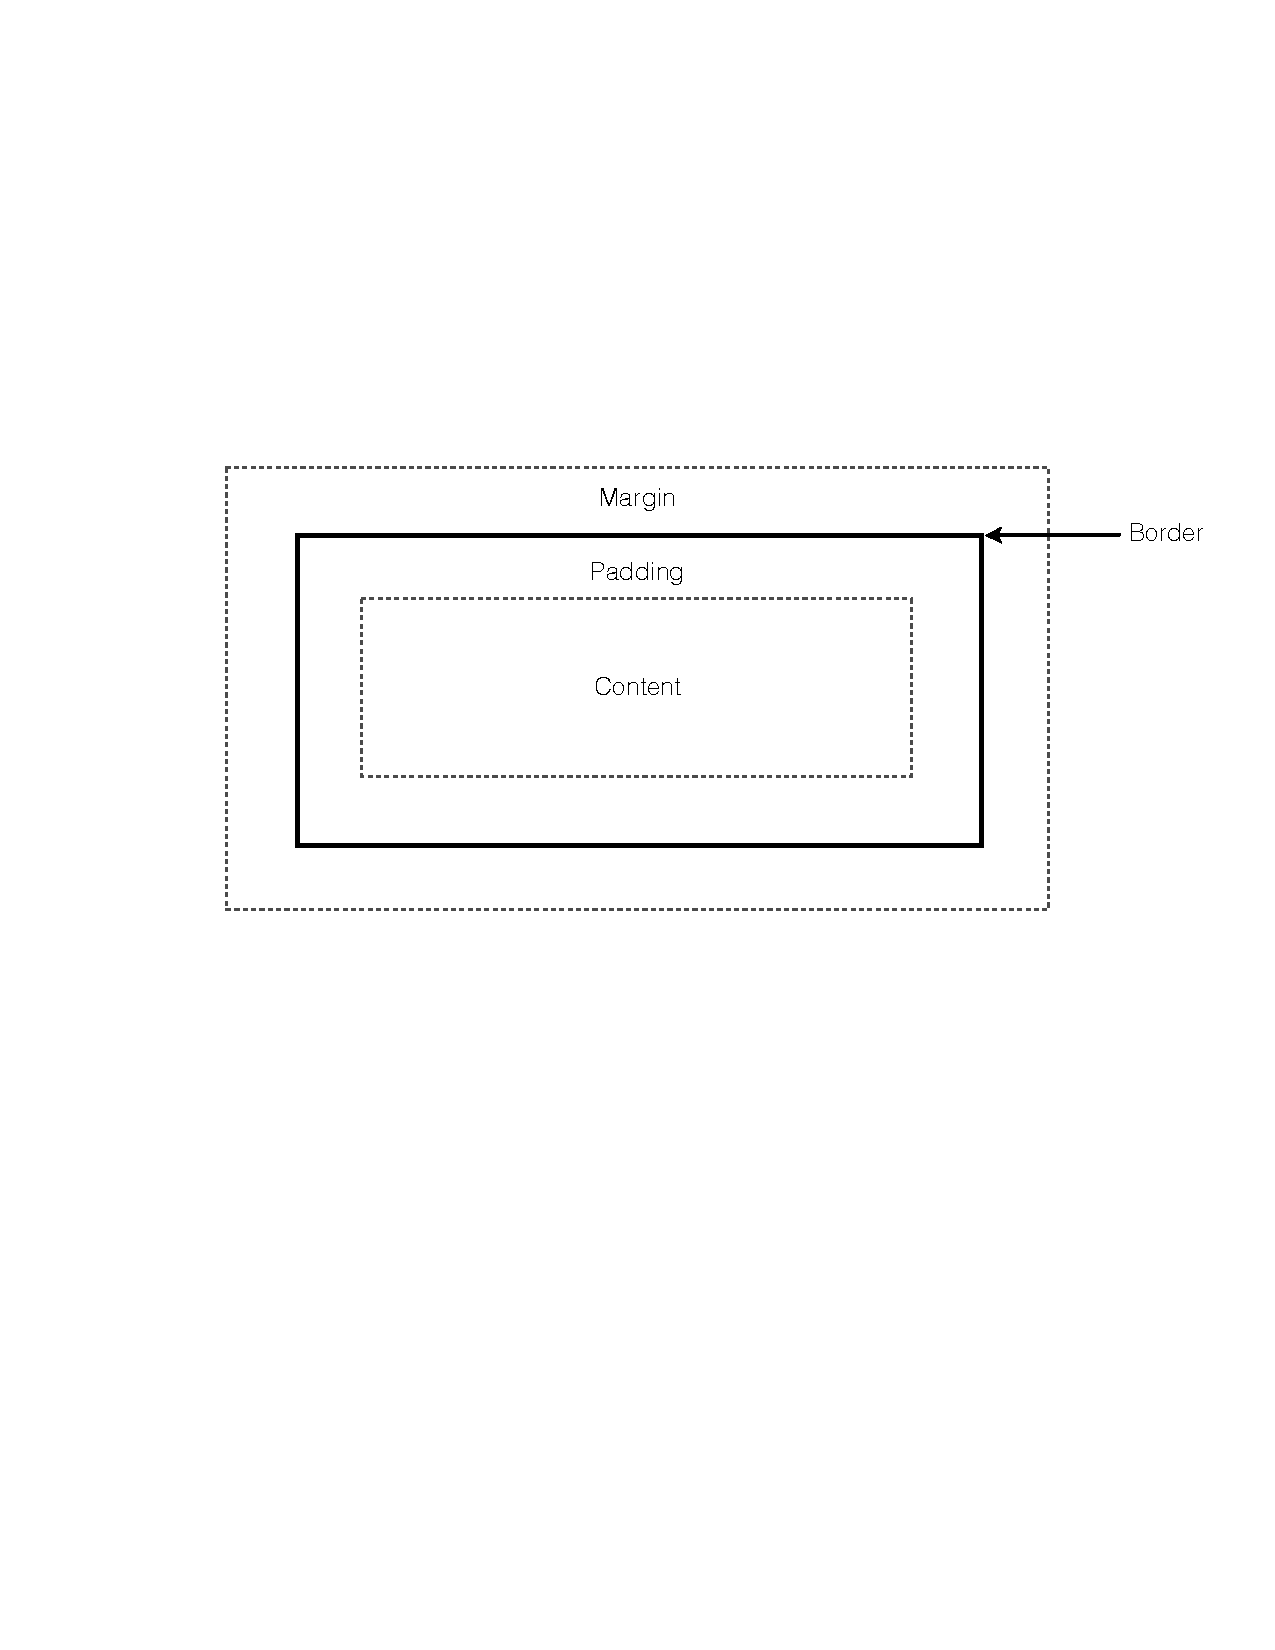
\includegraphics[width=\textwidth]{box_model}
	\caption{The Box Model}
	\label{fig:box_model}
\end{figure}

One should use \emph{margin} when spacing between elements is desired, and if one would like spacing from the content of the element to the border of the element, \emph{padding} should be used.



